\documentclass[a4paper, 11pt]{article}
\usepackage{comment}
\usepackage{amsmath}
\usepackage{mathtools}
\usepackage{fullpage}
\usepackage{graphicx}
\graphicspath{ {images/} }
\begin{document}
\title{Project proposal (CSE 519): Ranking arXiv papers}

\author{Amol Damare \\ adamare@cs.stonybrook.edu \\SBU ID: 107914028
\and
Punit Mehta \\  pmmehta@cs.stonybrook.edu \\SBU ID: 111461860}
\maketitle
\section{Introduction}
Researchers in various fields often present the findings of their research through either presenting a paper in a conference or publishing it in a journal. There are a lot of scientific papers published everyday. In the research community, `arXiv.org' is a central repository of electronic pre-prints of such papers. There are many research areas available in arXiv such as physics, mathematics, computer science, nonlinear sciences, quantitative biology, quantitative finance, statistics, electrical engineering and systems science, economics etc.  Everyday researchers publish their papers and upload pre-prints on arXiv.org.  It is not a trivial task to judge these papers even for an expert in a particular research area. An automated way to evaluate these papers and ranking them would be very useful. Such a ranking can be used to determine not only the best papers but also it can be used in other applications such as recommendation of papers, determining the key characteristics of a good paper etc. We want to tackle this problem during our course project for CSE 519 (Data science fundamentals). In this proposal, we will identify three key components of the problem statements. We will also give description of the data that we are going to use and present preliminary findings from our exploratory analysis of the data.  Finally, we will describe the approach we will be using to solve each component of the problems and propose our evaluation strategies. In the next section, we will review some of the work that is already done in this field.

\section{Related Works}
There has been a lot of work done in the field of ranking. Most important from our perspective is h-index proposed by \cite{Hirsch}. The h-index gives the ranking for researchers depending upon the number of papers published and citations received by these papers.
Similarly, there is a method based on g-index proposed in \cite{gindex} that also uses citations to rank the work of a researcher. There are other ranking algorithms that rank objects other than researcher or researcher's work. Most famous example of such ranking would be PageRank algorithm \cite{pagerank}. Other significant works in this area include Citation Analysis by E. Garfield \cite{garfield}, and work by Pinski and Narin \cite{pinski} wherein they found that not every citation is equal and developed a ranking that will incorporate this key concept.

\section{Problem Statement}
The goal of this project is to analyze all the scientific papers available on arXiv.org and come up with a ranking/scoring system that will give an estimate on how good the paper is. Specifically, we have identified the following three key components (sub-problems) that we will try to solve.
\begin{enumerate}
\item Ranking the papers which are already published and are available on arXiv.
\item Ranking the papers which are not published anywhere but available on arXiv from quite some time.
\item Ranking new papers which are recently uploaded on arXiv and are not published or accepted anywhere yet.
\end{enumerate}

In the first sub-problem, we will consider the papers which have been accepted by a conference or have been published in a journal. Depending upon quality of the paper, these papers will have a good number of citations. 

In the second sub-problem, we will consider papers for which we have pre-prints on arXiv.org for a relatively longer time but they are not published or presented at any conference/journal due to reasons unknown. These kind of papers may or may not have citations.

In the last sub-problem, we will consider papers that are relatively new and are not published anywhere. For these papers we will most probably will not have citations. Next section, we will describe the data in detail.

\section{Data}

\begin{figure}[h]
    \centering
    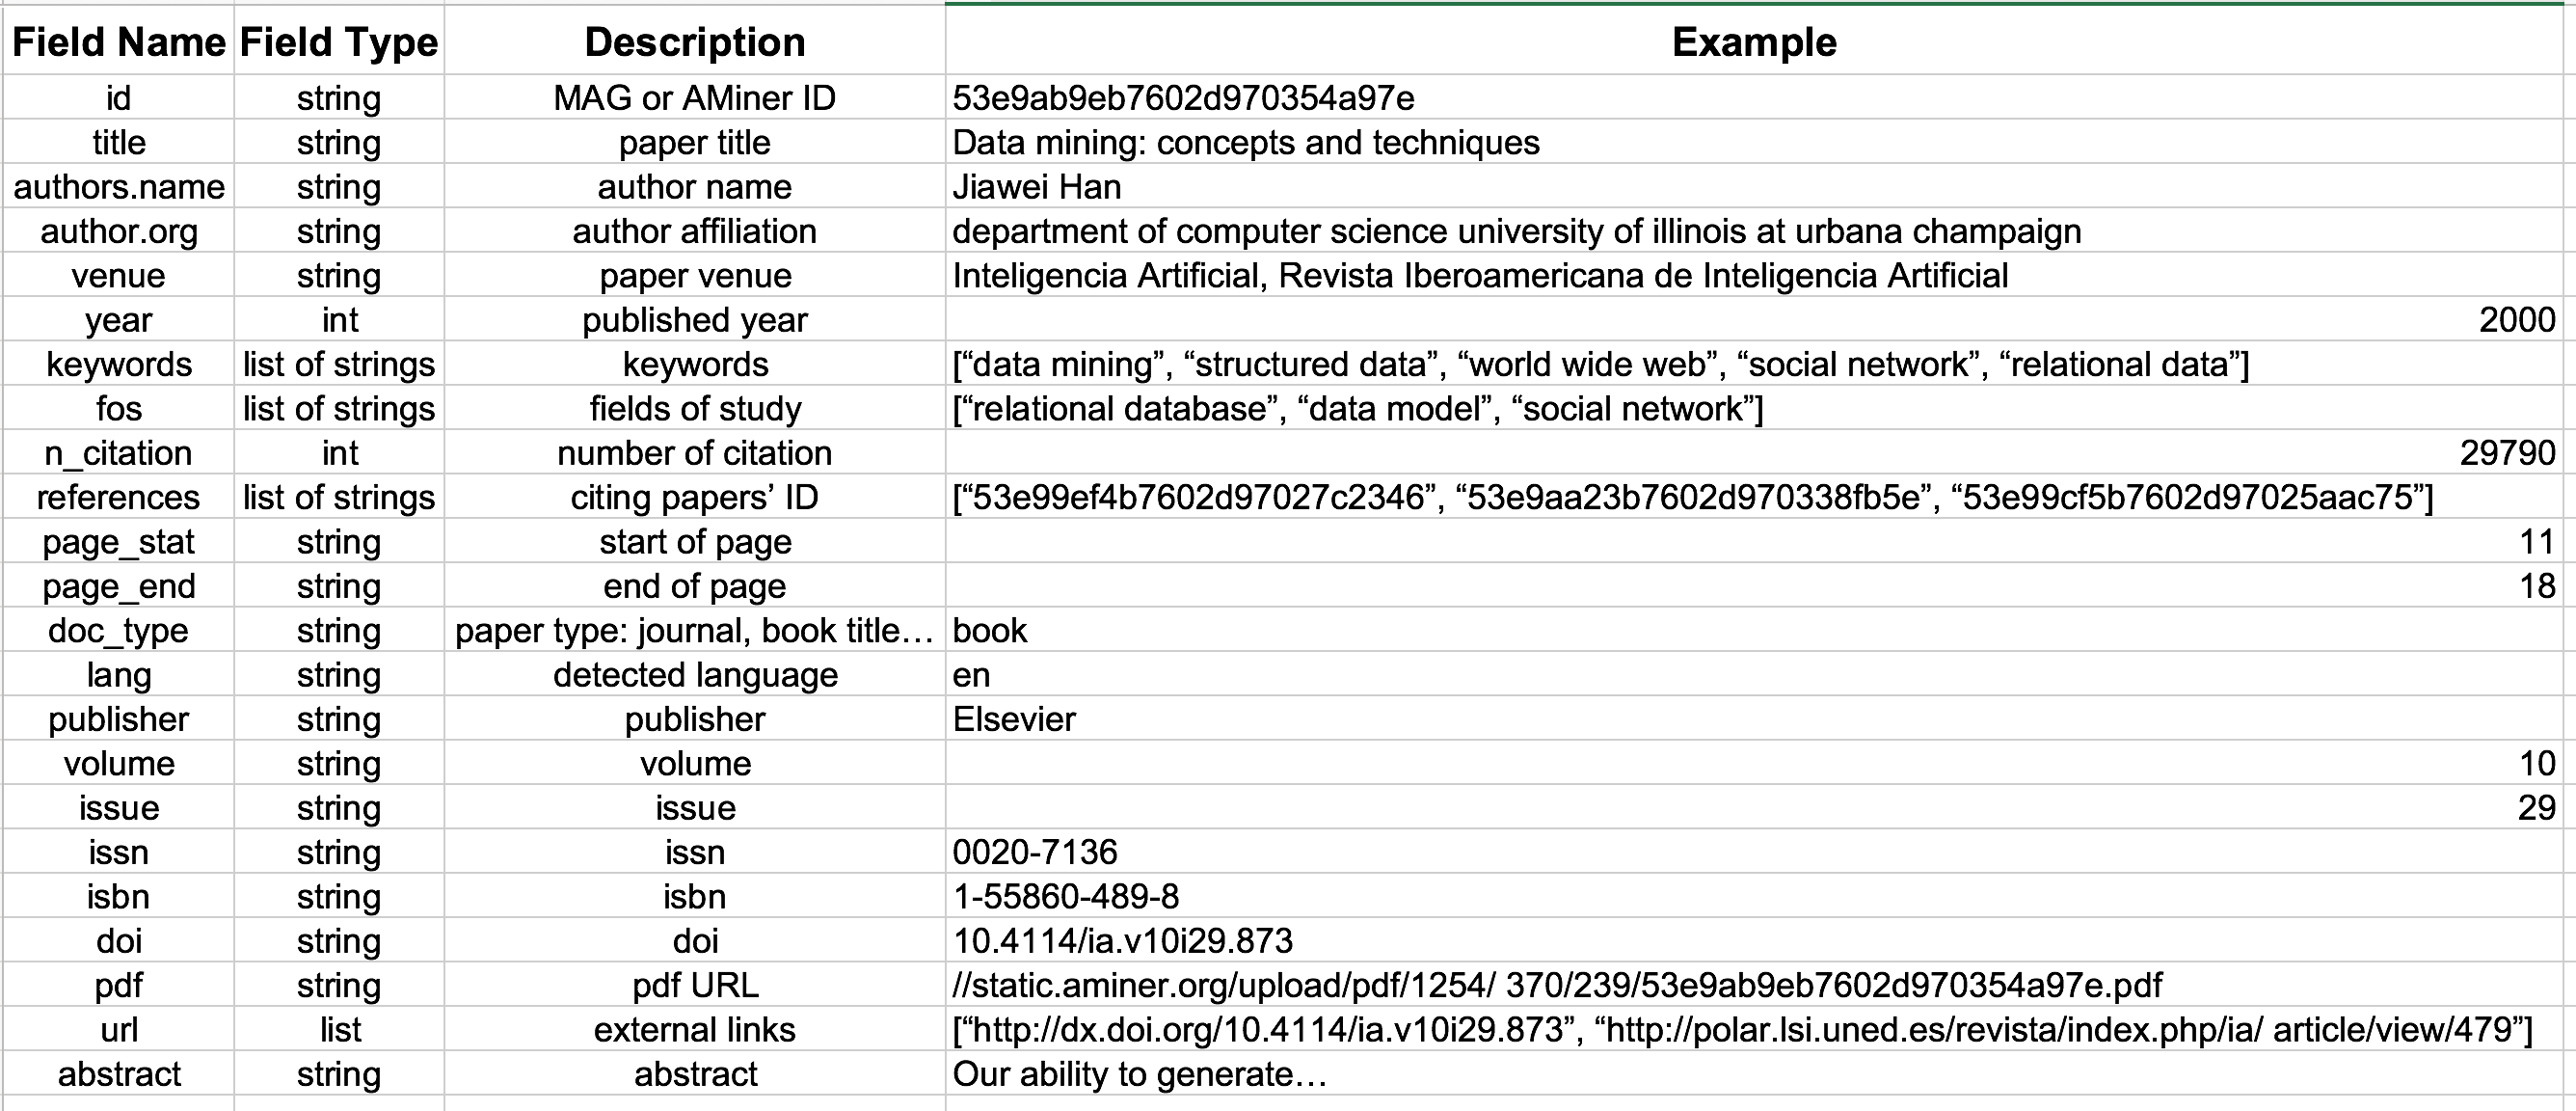
\includegraphics[width=17cm,height=8cm]{datamodel_new}
    \caption{Paper data model and its fields \cite{data}}
    \label{fig:datamodel}
\end{figure}

\begin{figure}[h]
    \centering
    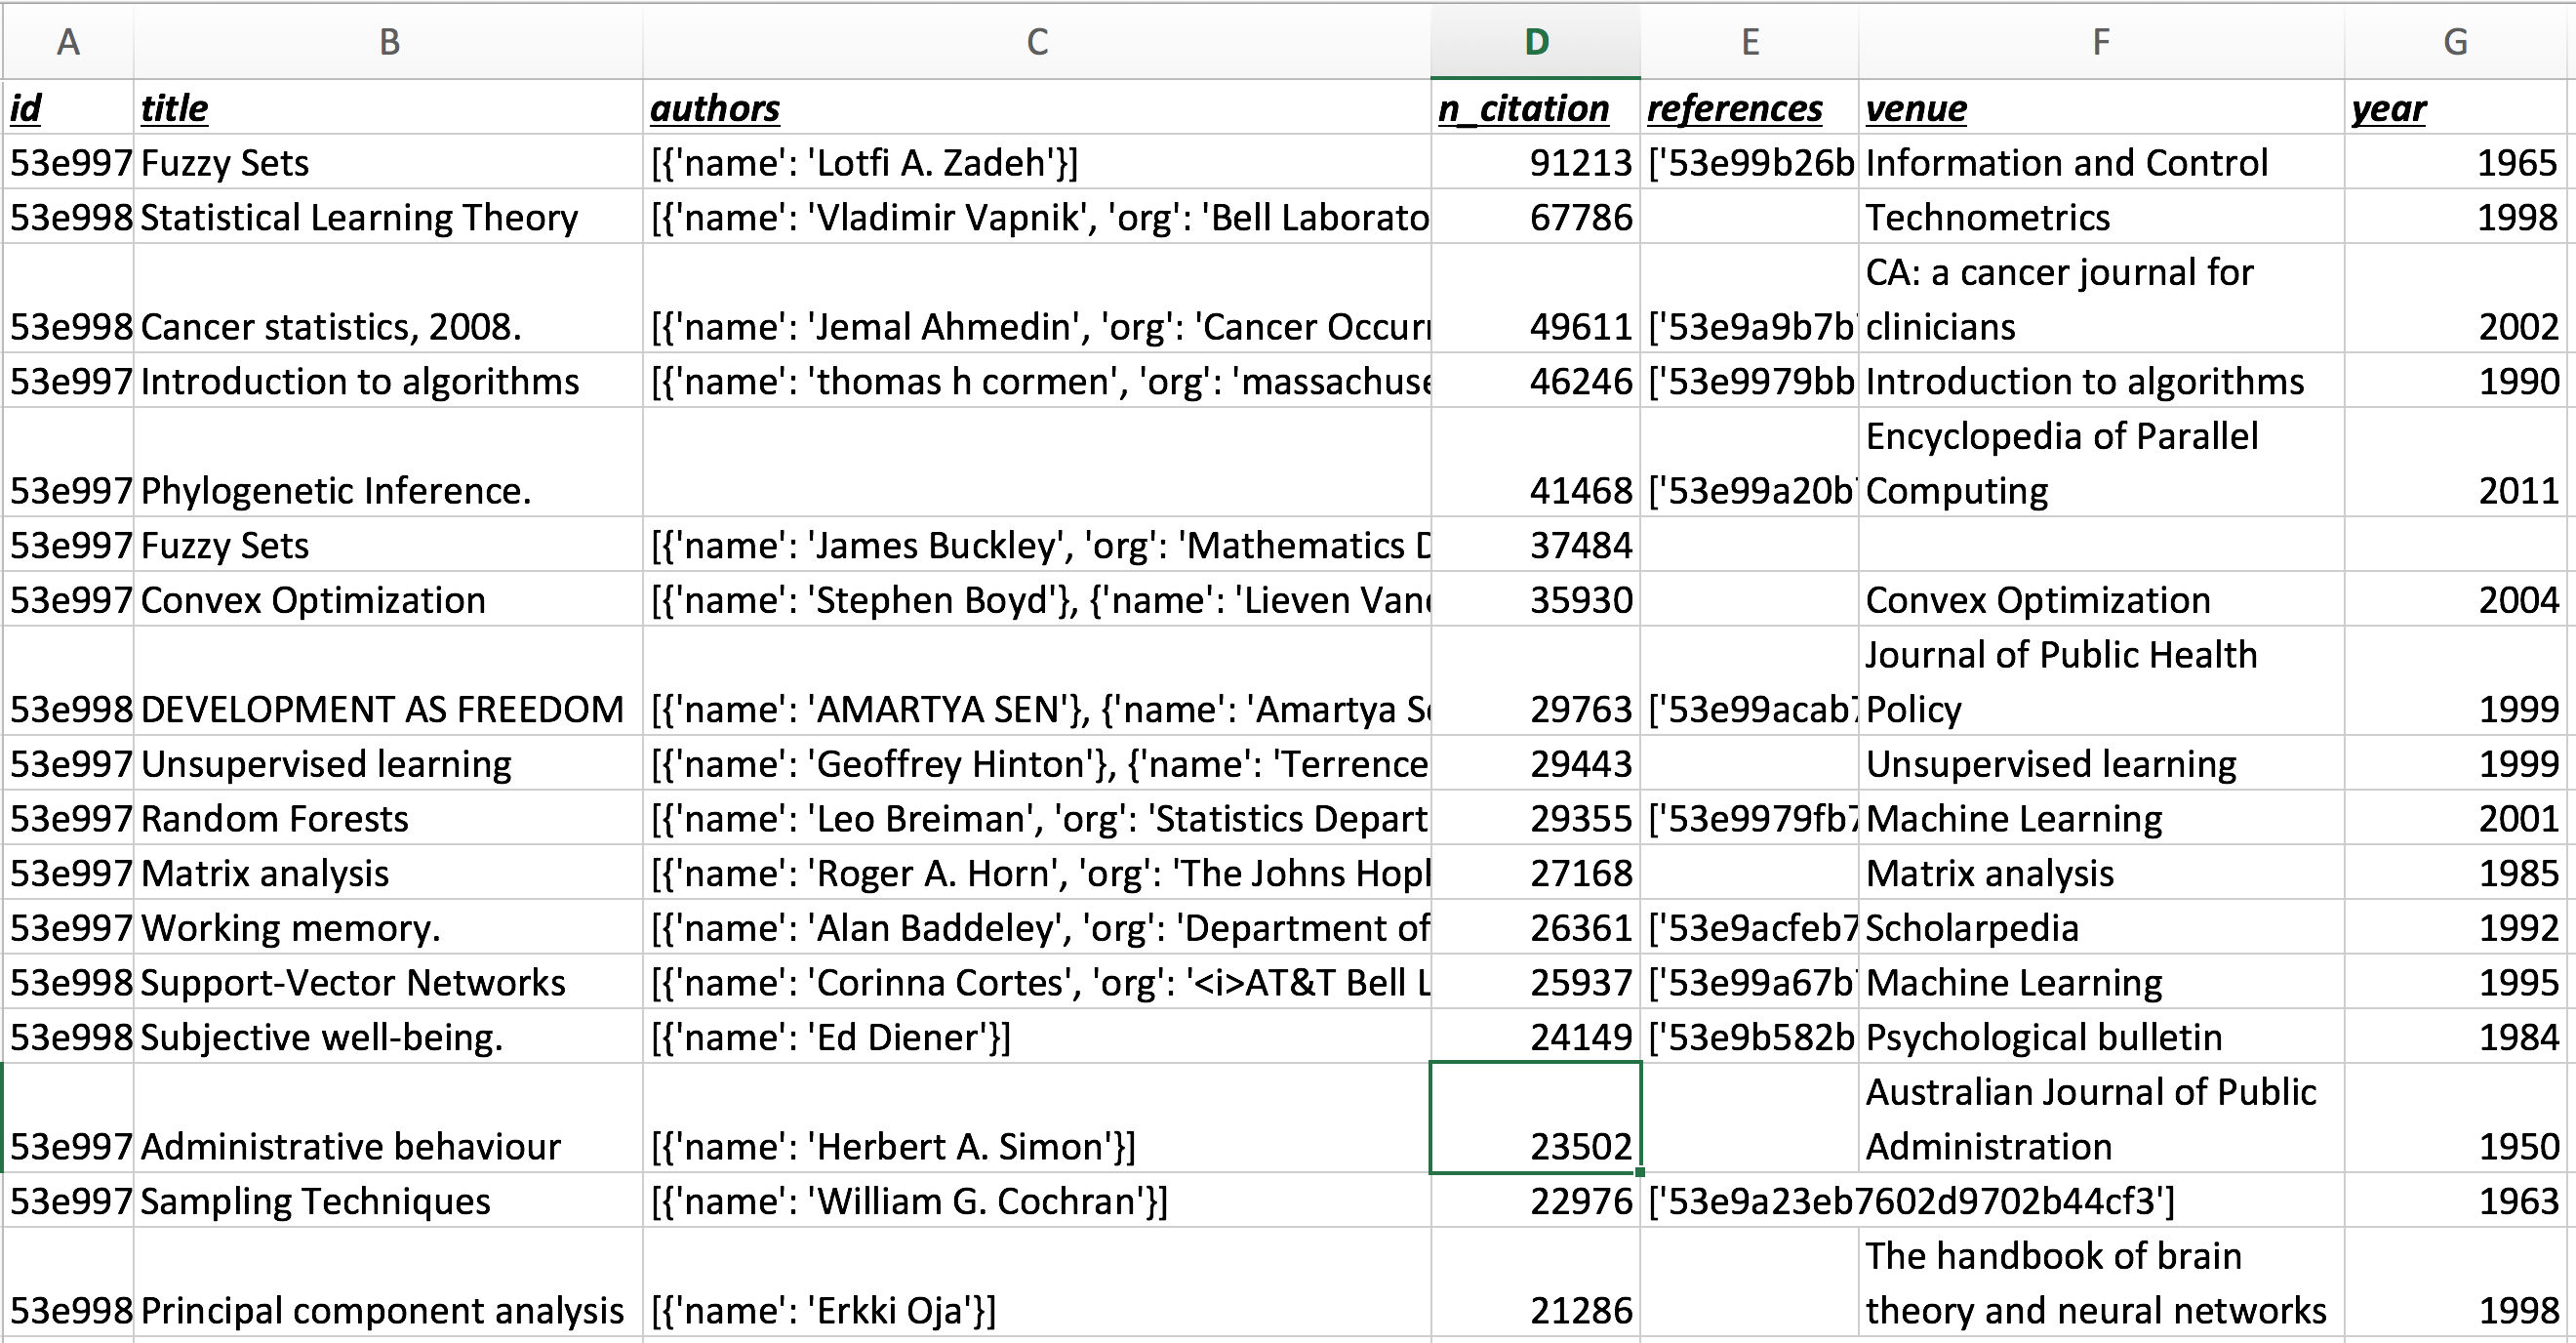
\includegraphics[width=17cm,height=9cm]{top_papers}
    \caption{Top records with max citations}
    \label{fig:top_papers}
\end{figure}

\begin{figure}[h]
    \centering
    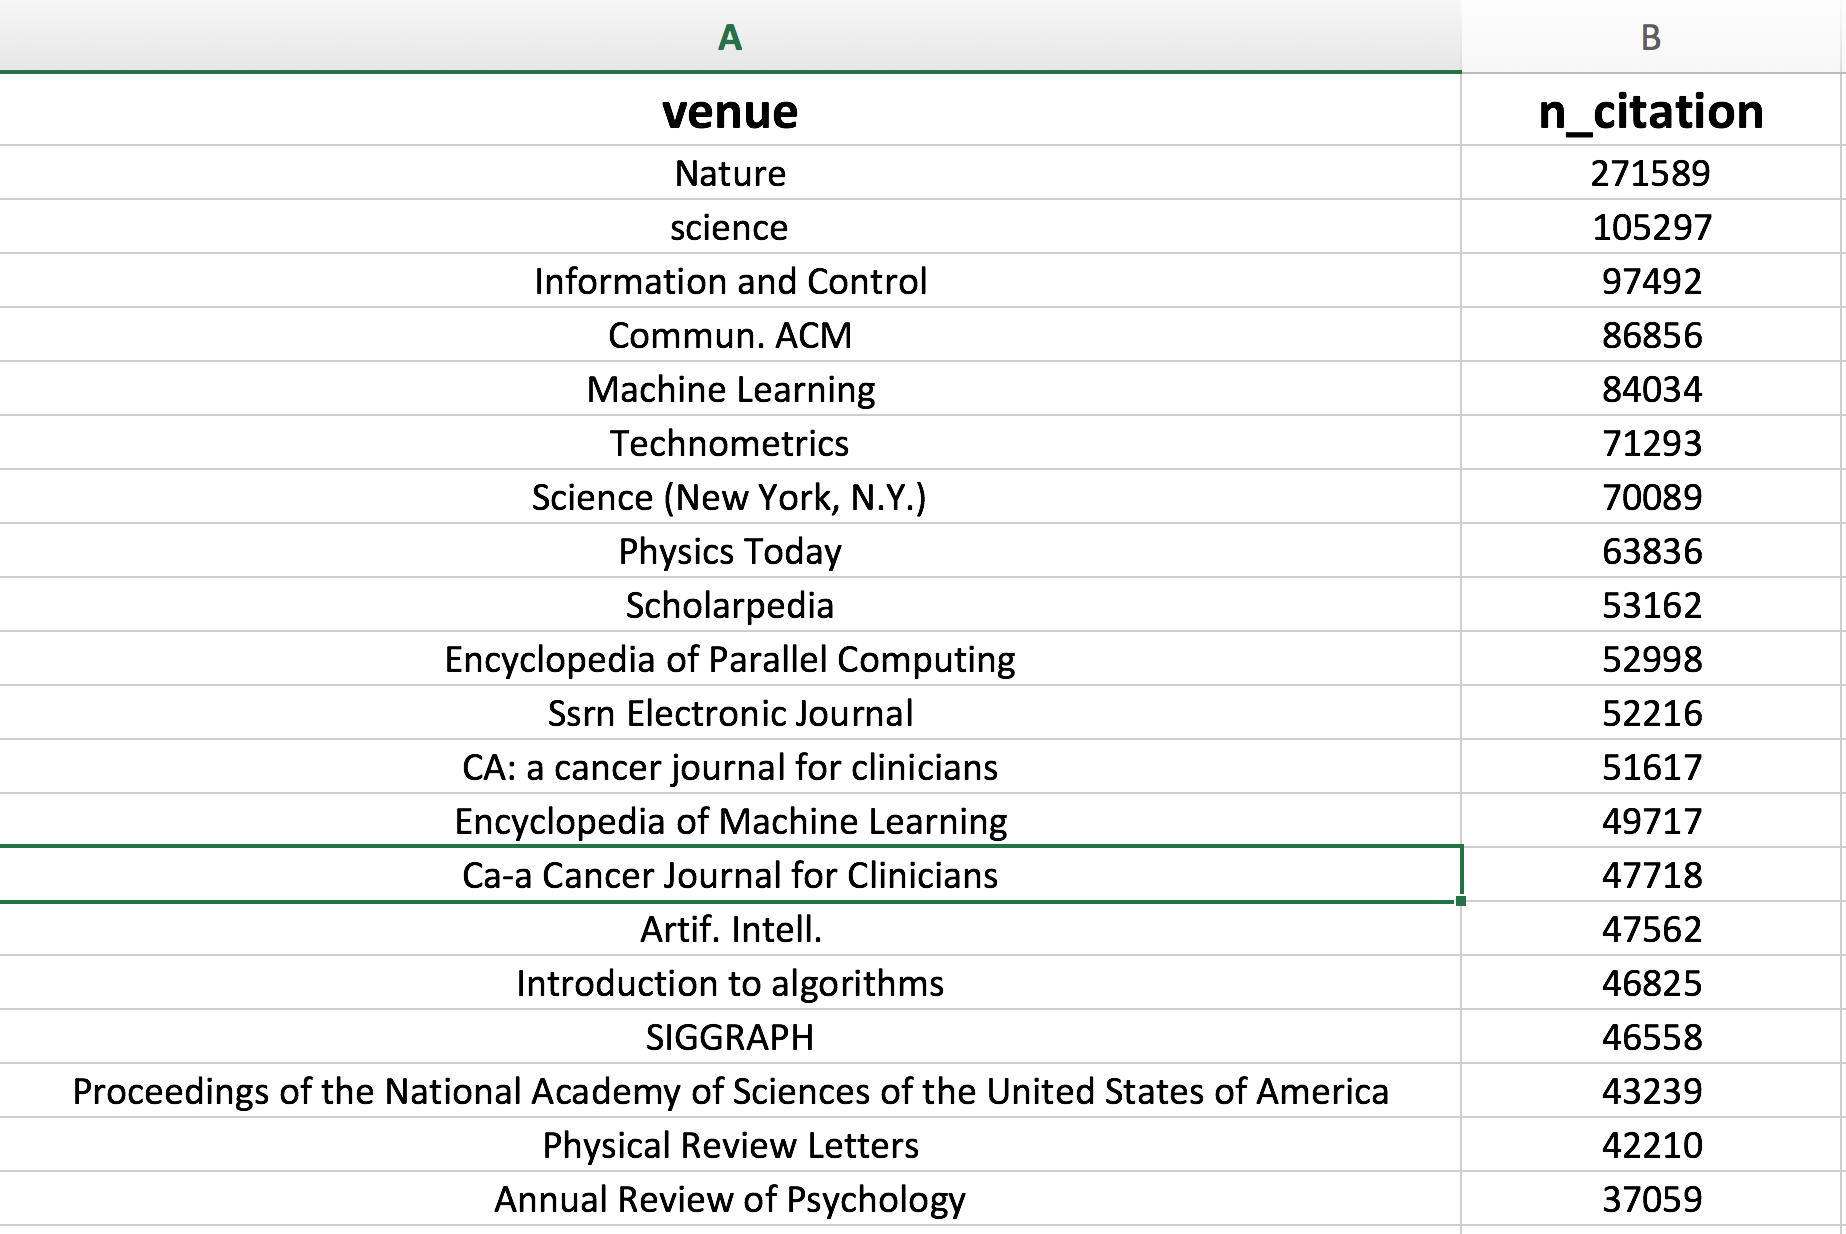
\includegraphics[width=17cm,height=11cm]{top_venues}
    \caption{Top venues with max citations}
    \label{fig:top_venues}
\end{figure}

\begin{figure}[h]
    \centering
    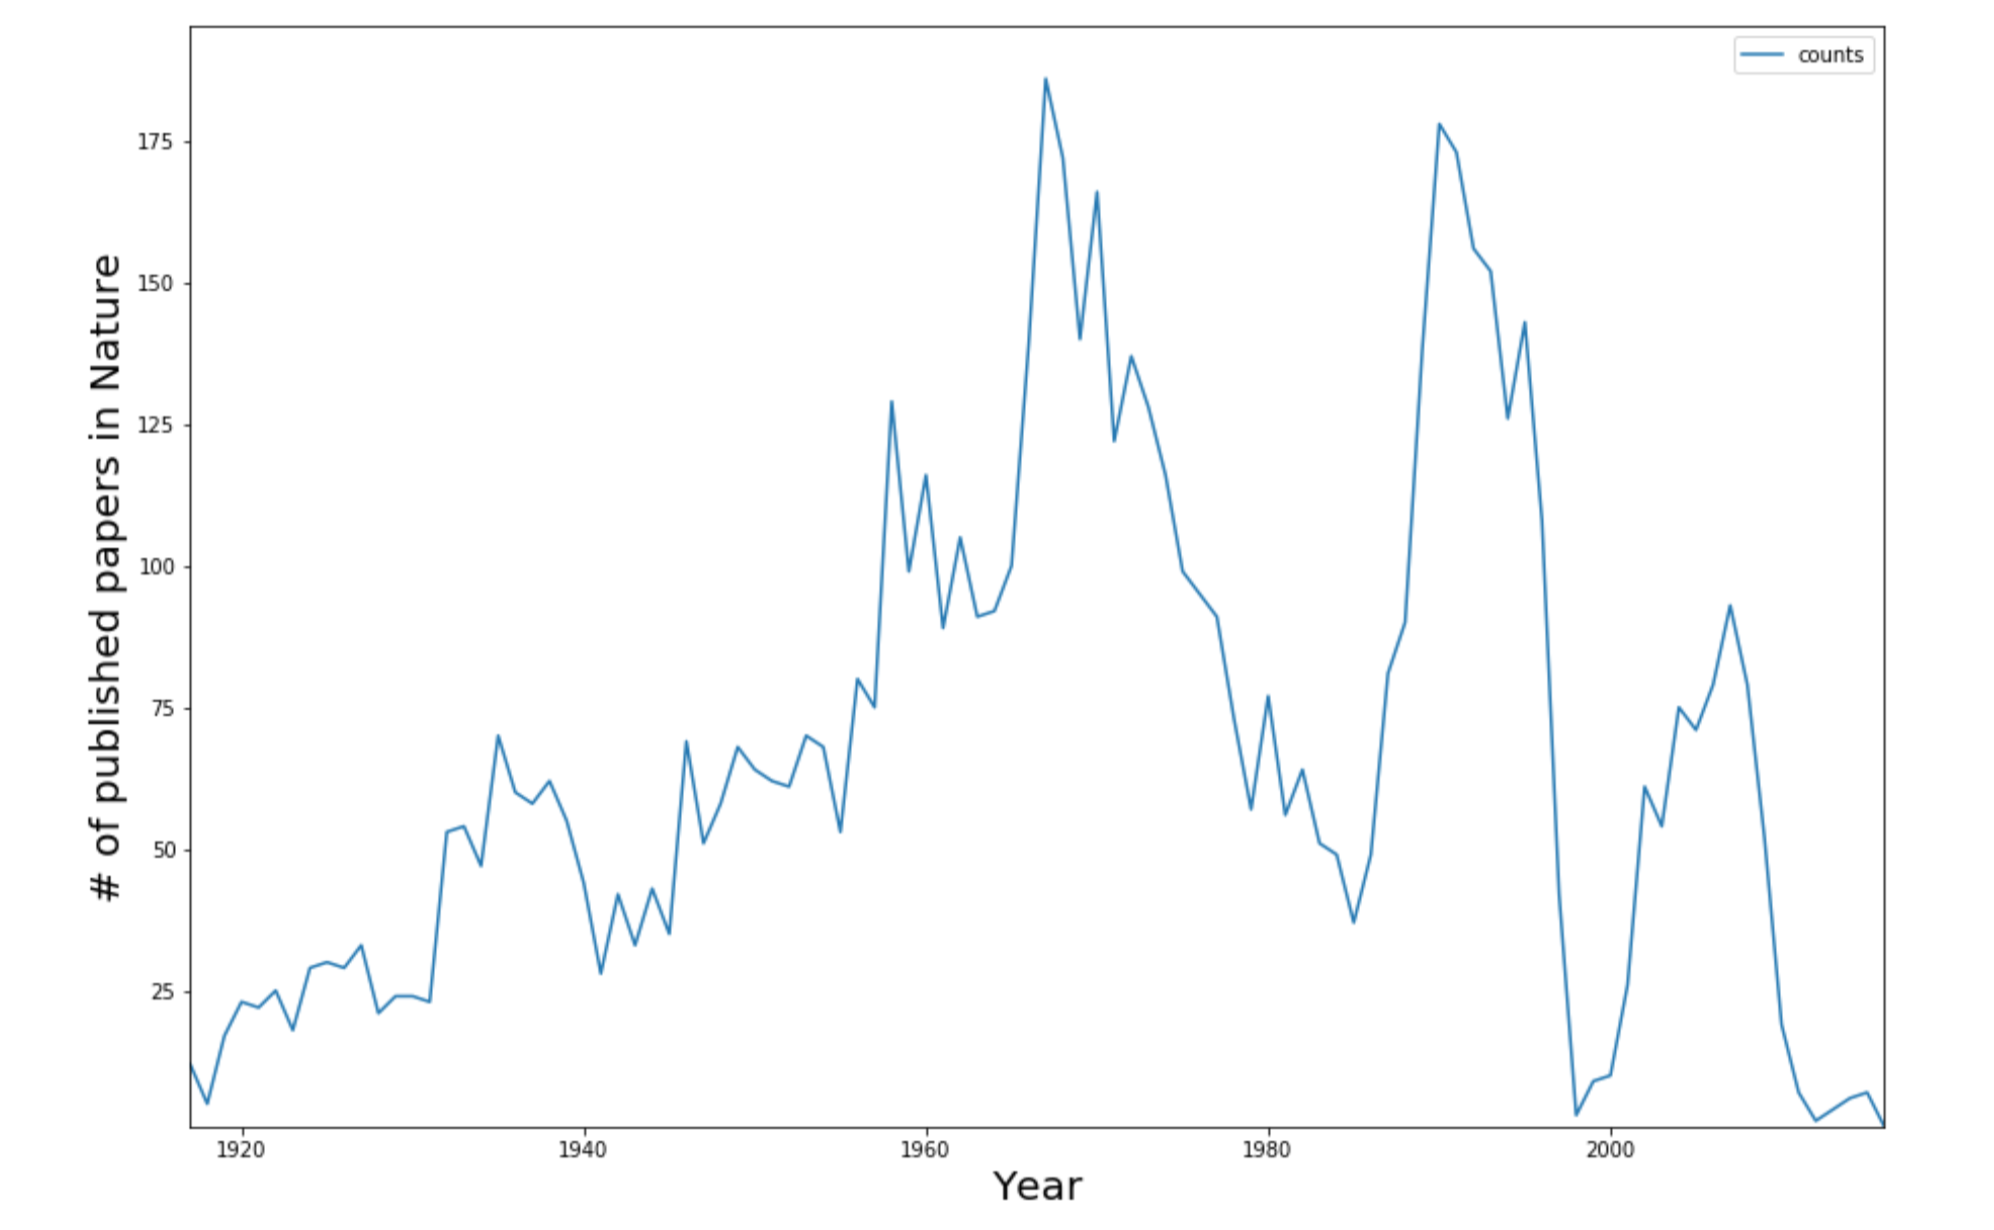
\includegraphics[width=17cm,height=11cm]{nature_year_wise}
    \caption{Papers published in Nature in last century}
    \label{fig:nature_year_wise}
\end{figure}

Following are the data sources that we have as of now and are planning to use for the project. 
\begin{enumerate}
\item All the pre-prints on arXiv.org are freely available. We can use the apis provided by arXiv.org to get all the data we need.  
\item Specifically, we will be needing data about the paper such as names of authors, paper's total citations, keywords, references and so on. We will also need data about its authors such as their number of papers, total number of citations, affiliated institutes etc. While exploring about the options to get this information, we found that Microsoft academic graph and open academic graph \cite{data} already crawl this information for arXiv as well as other sources. A snapshot of this data is freely available. We are mainly going to use this data for the purpose of this project. We played with their json data files using panda data-frame and following are our initial observations and findings.

Figure \ref{fig:datamodel} shows the fields available for each of the paper. It includes abstract of the paper, link to author objects , links to the reference papers, keywords etc. 

Figure \ref{fig:top_papers} shows some of the top records (having maximum citations) that we found after some data-frame processing.

Similarly, figure \ref{fig:top_venues} lists the top venues with the total number of citations. Clearly, Nature and Science are the most popular in scientific community. 

Figure \ref{fig:nature_year_wise} shows the number of papers publised in Nature in the last 100 years. The data we used to plot this is from one of the data files (and not the entire database as it's distributed across files) and it's not fair to conclude anything based on this graph at this moment as there is a lot of more data to be processed.
\item Scirate \cite{scirate} is a platform that shows the top papers for varieties of fields. It's mentioned on their portal that the data is available under Creative Common License. So, we have requested them to give access to the data and we hope that we will get it. With the help of Scirate, we can even tune our model better according to our use-cases.
\end{enumerate}




\section{Our Approach and Evaluation criteria}
\subsection{Approach}
Judging a scientific paper is a hard task even for an expert. But there are some heuristics that can help in estimating the quality of a paper. For example, we know that a particular author generally writes good papers and hence, probability of a new paper by the same author being good is very high. Another heuristic is citations. If a paper is referenced in a lot of other papers then we can safely assume that it will be a good paper. \cite{Hirsch} \cite{pinski} have presented ideas based on the citations. But we can not get a generalized scoring function from citations alone because number of citations depends upon the field that is, if the research in the field is difficult in general, papers in that field will have less citations. Additionally, if there are few number of people working in that field, number of total citations per paper will be low. Hence, number of citations alone can not be used to estimate the quality of a paper. Other factor that needs to be considered is a rank of the conferences or journals where the paper was published. In general, if paper is published in a good conference, it will be a good paper.  When experts are reviewing scientific papers, they usually have some criteria from which they can determine the quality of a paper. For example, a good paper generally has about eight pages (or page limits for most of the conferences) with one page of introduction and one page of related section. It should have some figures or some kind of experiment section, a technical section with mathematical proof etc \cite{karpathy}.  
\par
To evaluate the quality of each paper, we will use impact of the author (may be h-index), number of citations, number of references, quality of references, field of study, affiliated institutes, conferences/journals published. In addition to these parameters, we will also extract features from paper itself such as number of pages, number of figures/tables etc. We are also thinking of extracting features using NLP (possibly by creating embeddings for papers) and using these features in our model. We hope to uncover more factors that will contribute to the estimate of the quality of a paper during the course of this project.
\subsection{Evaluation Criteria}
Keeping in mind the above approaches and our three sub-parts of the main problem statement, we have the following evaluation criteria for each of the sub-problem.
\begin{enumerate}
\item  For first sub-problem, we will have most amount of information since we are considering the papers that are accepted in a conference or published in a journal. We can calculate the score by getting the conference levels wherein the paper is published, citations of the paper, impact of the authors, affiliation details and other parameters which we will extract from the text of the paper

\item We have little less information in the second sub-problem than the first since we are considering papers which are not published anywhere. For unpublished papers which are available from quite some time, we assume that if they are good, they will have a good number of citations. We can take such papers, evaluate our model and if they are good, our model should give positive results.

\item In this case, we have the least amount of information and evaluation is also hard. For new papers, we will not have citations or any other external data to score it. In this case, we will mostly use the details available in the paper (that is authors' details, references and their credibility, number of pages, a proper format with relevant titles, figures etc.). We found one good resource \cite{scirate}  that already classifies good arxiv paper up to some extent and we can get the top papers from there (which will be very recent) and can evaluate our model by comparing it.
\end{enumerate}

\section{Conclusion}
TODO
\begin{thebibliography}{9}
\bibitem{Hirsch}
J. E. Hirsch.
\newblock An index to quantify an individual's scientific research output, 2005,
\newblock Proc.Nat.Acad.Sci.46:16569,2005;
\newblock arXiv:physics/0508025.
\newblock DOI: 10.1073/pnas.0507655102.
\bibitem{gindex}
Egghe, L.
\newblock  Theory and practise of the g-index
\newblock Scientometrics (2006) 69: 131.
\newblock https://doi.org/10.1007/s11192-006-0144-7
\bibitem{pagerank}
Page, L., Brin, S., Motwani, R., Winograd, T. 
\newblock  The PageRank citation ranking: Bringing order to the web  
\newblock  (Technical Report). Stanford InfoLab.
\bibitem{garfield}
Garfield, E.
\newblock  Citation analysis as a tool in journal evaluation
\newblock Science,178,471-479.
\bibitem{pinski}
Pinski, G.,  Narin, F. 
\newblock Citation influence for journal aggregates of scientific publications: Theory, with application to the literature of physics
\newblock  Information Processing and Management, 12(5), 297-312
\bibitem{data}
Microsoft Academic Graph 
\newblock https://www.openacademic.ai/oag/
\bibitem{karpathy}
Andrej Karpathy blog
\newblock http://karpathy.github.io/2016/09/07/phd/
\newblock "Writing paper" section
\bibitem{scirate}
SciRate.org
\newblock  https://scirate.com/arxiv/stat.ML
\bibitem{arxiv}
arXiv.org
\newblock  https://arxiv.org/

\end{thebibliography}

\listoffigures

\end{document}
